\section{Results}

\label{sec:results}

The effectiveness of the proposed approach is illustrated using the Synthea dataset, which is introduced in Section~\ref{sec:system}. Out of 22{,}284 patients, only 21{,}995 patients have been clustered, and all outliers have been retained in a different class labeled as $-1$.

\subsection{Clustering}

To discover the optimal configuration, we performed a huge benchmarking procedure on 629 configurations. Configuration means feature subset selection (we tried more than sixty feature subsets), cluster number $k$, scaler used, categorical weight $\gamma$, random state and outlier threshold. For benchmarking, we calculated a score based on three metrics. First of all, the metrics are min-max normalized individually within the scope of all 629 configurations, and the score is then their linear combination with weights that reflect our confidence in them ($0.5$ for Gower silhouette, $0.3$ for Calinski-Harabasz index and $0.2$ for Davies-Bouldin index, inverted because the higher the score the worse the partition is). We chose the best clinically interesting configuration per $k$ value (we tried four, five and six), and from these three configurations we tried once again to optimize the hyperparameters and feature subset used in order to choose the best local configuration.

\begin{table*}[t]

\caption{Representative clustering configuration for each cluster number (feature vector based on the corresponding version id). CH index and DB index are computed from the FAMD embedding in the mixed score framework. The highest value obtained for each criterion is marked in bold font. The selected cluster number is $k=4$ (v55).}

\label{tab:clusters}

\centering

\footnotesize

\begin{tabular}{@{}l c c l c r c@{}}

\toprule

Config & $k$ & Gower & Per-cluster Gower & DB & CH & Score \\

\midrule

v55 (final) & 4 & \textbf{0.350} & 0.42, 0.20, 0.32, 0.40 & \textbf{0.72} & \textbf{26813} & \textbf{0.82} \\

v40 & 5 & 0.324 & 0.28, 0.22, 0.31, 0.19, 0.48 & 0.87 & 22547 & 0.74 \\

v60 & 6 & 0.287 & 0.17, 0.13, 0.47, 0.21, 0.38, 0.27 & 0.95 & 22273 & 0.70 \\

\bottomrule

\end{tabular}

\end{table*}

Table~\ref{tab:clusters} reports a representative configuration for each $k$. The choice of $k$ is made to be 4, with feature combination v55. It scores best overall (0.82) among the clinically meaningful runs, and does so across all individual metrics: the largest Gower silhouette, the largest Calinski-Harabasz score, and the smallest Davies-Bouldin score. We still eliminate one family of runs, which scores even better on paper. It achieves a score of 0.87 by segregating patients according to gender, but since the separation is meaningless clinically, we exclude them. Among the four clusters in the optimal run, three get a Gower silhouette per cluster greater than 0.30, and only one gets close to 0.20, compared with the results of five and six clusters where one and two clusters respectively have values less than 0.20. Since clusters will be used for the scope of the sequence mining analysis, we prefer to have the smallest $k$ possible while still having all the clusters be cohesive. The important features are the number of active conditions and patient age numerically, and condition burden, gender, diabetes, and heart disease categorically.

Figure~\ref{fig:heatmap} shows the per-cluster means of the numeric variables represented as a heatmap. There is certainly a morbidity gradient. That is, cluster 0 represents young people with low morbidity, while the rest of the clusters contain a progressively greater number of conditions. By interpreting all four clusters in conjunction with the categorical features, we see four distinct patient profiles, which the AI platform automatically labels as: Younger Injury Care (young, low morbidity), Pregnancy Focused Adults (reproductive women), Older High Risk (hypertensive polypharmacy adults), and Kids and Well Visits (pediatric/acute patients).

\begin{figure}[t]

\centering

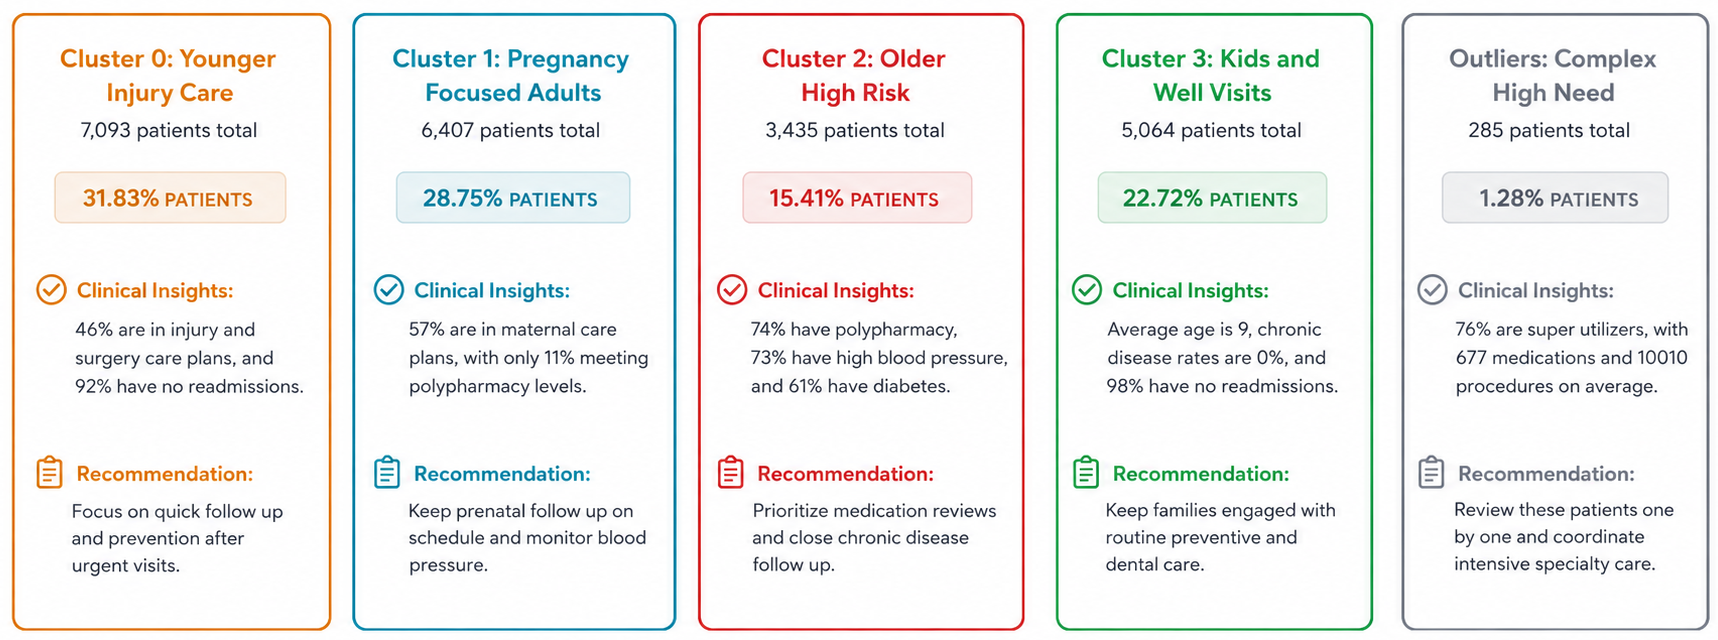
\includegraphics[width=0.95\linewidth]{figs/cluster_heatmap.png}

\caption{Z-scored numerical feature means per cluster ($k=4$). Warm colours are above the population average, cool colours below it.}

\label{fig:heatmap}

\end{figure}

\subsection{Sequence Mining}

The most straightforward demonstration of the impact of our pipeline can be seen through the transformation in the properties of the mined patterns as each new version is introduced. In Table~\ref{tab:ablation}, we present two sample patterns of at least four events from every one of these versions. The initial versions (v0-v2) rank patterns solely based on support, and therefore, the beginning of the ranking consists of common yet meaningless sequences, which consist mainly of similar dental cleanings that about 93\% of the patients undergo. With v3 and onwards, geometric mean lift-based ranking along with diversity filters were applied, and at the top of the ranking, clinically consistent care pathways can be seen. Version v4 also filters out consecutive occurrence of similar events, which is why the long sequence of procedure events related to a diabetic eye exam no longer appears from v4 onwards. At v6, when social status events are removed and reserved space for full spectrum patterns was set aside, diverse combinations of conditions, care plans, medicines and procedures appear despite their low support scores.

\begin{table}[t]

\caption{How the mined patterns evolve across miner versions}

\label{tab:ablation}

\centering

\scriptsize

\begin{tabular}{@{}l p{0.72\linewidth} r@{}}

\toprule

Ver. & Example pattern (length $\ge 4$) & Sup. \\

\midrule

v0 & dental consultation $\rightarrow$ dental care $\rightarrow$ supragingival scaling $\rightarrow$ subgingival scaling & 93\% \\

v0 & supragingival scaling $\rightarrow$ subgingival scaling $\rightarrow$ gingivae exam $\rightarrow$ oral health education & 93\% \\

\addlinespace

v1 & supragingival scaling $\rightarrow$ subgingival scaling $\rightarrow$ gingivae exam $\rightarrow$ oral health education & 63\% \\

v1 & dental care $\rightarrow$ supragingival scaling $\rightarrow$ subgingival scaling $\rightarrow$ oral health education & 63\% \\

\addlinespace

v2 & dental consultation $\rightarrow$ dental care $\rightarrow$ subgingival scaling $\rightarrow$ gingivae exam $\rightarrow$ oral health education & 62\% \\

v2 & dental referral $\rightarrow$ dental consultation $\rightarrow$ dental care $\rightarrow$ subgingival scaling $\rightarrow$ oral health education & 57\% \\

\midrule

v3 & tropicamide eye drops $\rightarrow$ gonioscopy $\rightarrow$ fundoscopy $\rightarrow$ diabetic eye exam & 3\% \\

v3 & furosemide $\rightarrow$ oxygen by mask $\rightarrow$ prone position $\rightarrow$ furosemide & 2\% \\

\addlinespace

v4 & acute bronchitis $\rightarrow$ respiratory therapy $\rightarrow$ respiratory function test $\rightarrow$ acetaminophen & 3\% \\

v4 & salmeterol-fluticasone inhaler $\rightarrow$ albuterol $\rightarrow$ spirometry $\rightarrow$ depression screening & 2\% \\

\addlinespace

v5 & subgingival scaling $\rightarrow$ gingivae exam $\rightarrow$ sodium fluoride gel $\rightarrow$ fluoride treatment & 35\% \\

v5 & dental bitewing X-ray $\rightarrow$ gingivae exam $\rightarrow$ sodium fluoride gel $\rightarrow$ fluoride treatment & 19\% \\

\addlinespace

v6 & acute bronchitis $\rightarrow$ respiratory therapy $\rightarrow$ respiratory function test $\rightarrow$ acetaminophen & 3\% \\

v6 & chest X-ray $\rightarrow$ furosemide $\rightarrow$ oxygen by mask $\rightarrow$ prone position $\rightarrow$ furosemide & 1\% \\

\bottomrule

\end{tabular}

\end{table}

Frequent pattern mining from each scope individually yields 175-252 frequent patterns per cluster. Examples of representative frequent patterns are listed in Table~\ref{tab:patterns}. Each cluster has a unique signal dominating its set of frequent patterns. For example, in Cluster~0, the dominant signal relates to acute care episodes. In Cluster~2, the chronic disease management includes antihypertensive drugs combined with screenings, or furosemide along with oxygen therapy to manage fluid overload. The most valuable benefit is obtained from the outlier scope. Since we mine each individual scope independently, high-cost combinations like chemotherapy and cisplatin leading to hospice care, or dialysis and epoetin, will dominate the results. Otherwise, these pathways fall under the global support threshold and would be missed when mining all cases at once.

\begin{table}[t]

\caption{Representative mined pathways by scope (ranked by GML).}

\label{tab:patterns}

\centering

\footnotesize

\begin{tabular}{@{}p{0.16\linewidth}p{0.74\linewidth}@{}}

\toprule

Scope & Pattern \\

\midrule

Cluster 0 & Fracture of bone $\rightarrow$ Fracture care $\rightarrow$ Bone immobilization \\

Cluster 1 & Normal pregnancy $\rightarrow$ Pregnancy test $\rightarrow$ Ultrasound for fetal viability \\

Cluster 2 & Furosemide $\rightarrow$ Oxygen by mask $\rightarrow$ Prone position $\rightarrow$ Furosemide \\

Cluster 3 & Acute allergic reaction $\rightarrow$ Epinephrine injection $\rightarrow$ Prednisone \\

Outliers ($-1$) & Chemotherapy + radiation $\rightarrow$ Cisplatin $\rightarrow$ Hospice care \\

\bottomrule

\end{tabular}

\end{table}

\subsection{AI Layer}

Upon running the K-Prototypes script, the AI creates a short card per cluster based on the statistics generated beforehand and determines the cluster title, its colour theme that will be used in all mentions of the cluster on the platform, its description, an insight and a recommendation for each. Figure~\ref{fig:platform_clusters} depicts how these cards look like in the dashboard. Since the model uses only the precomputed values, the card matches the heatmap and the prevalence rates by assigning high risk and a cardiology-related recommendation to the high-burden cluster, and a healthy, preventive profile otherwise.

\begin{figure}[t]

\centering

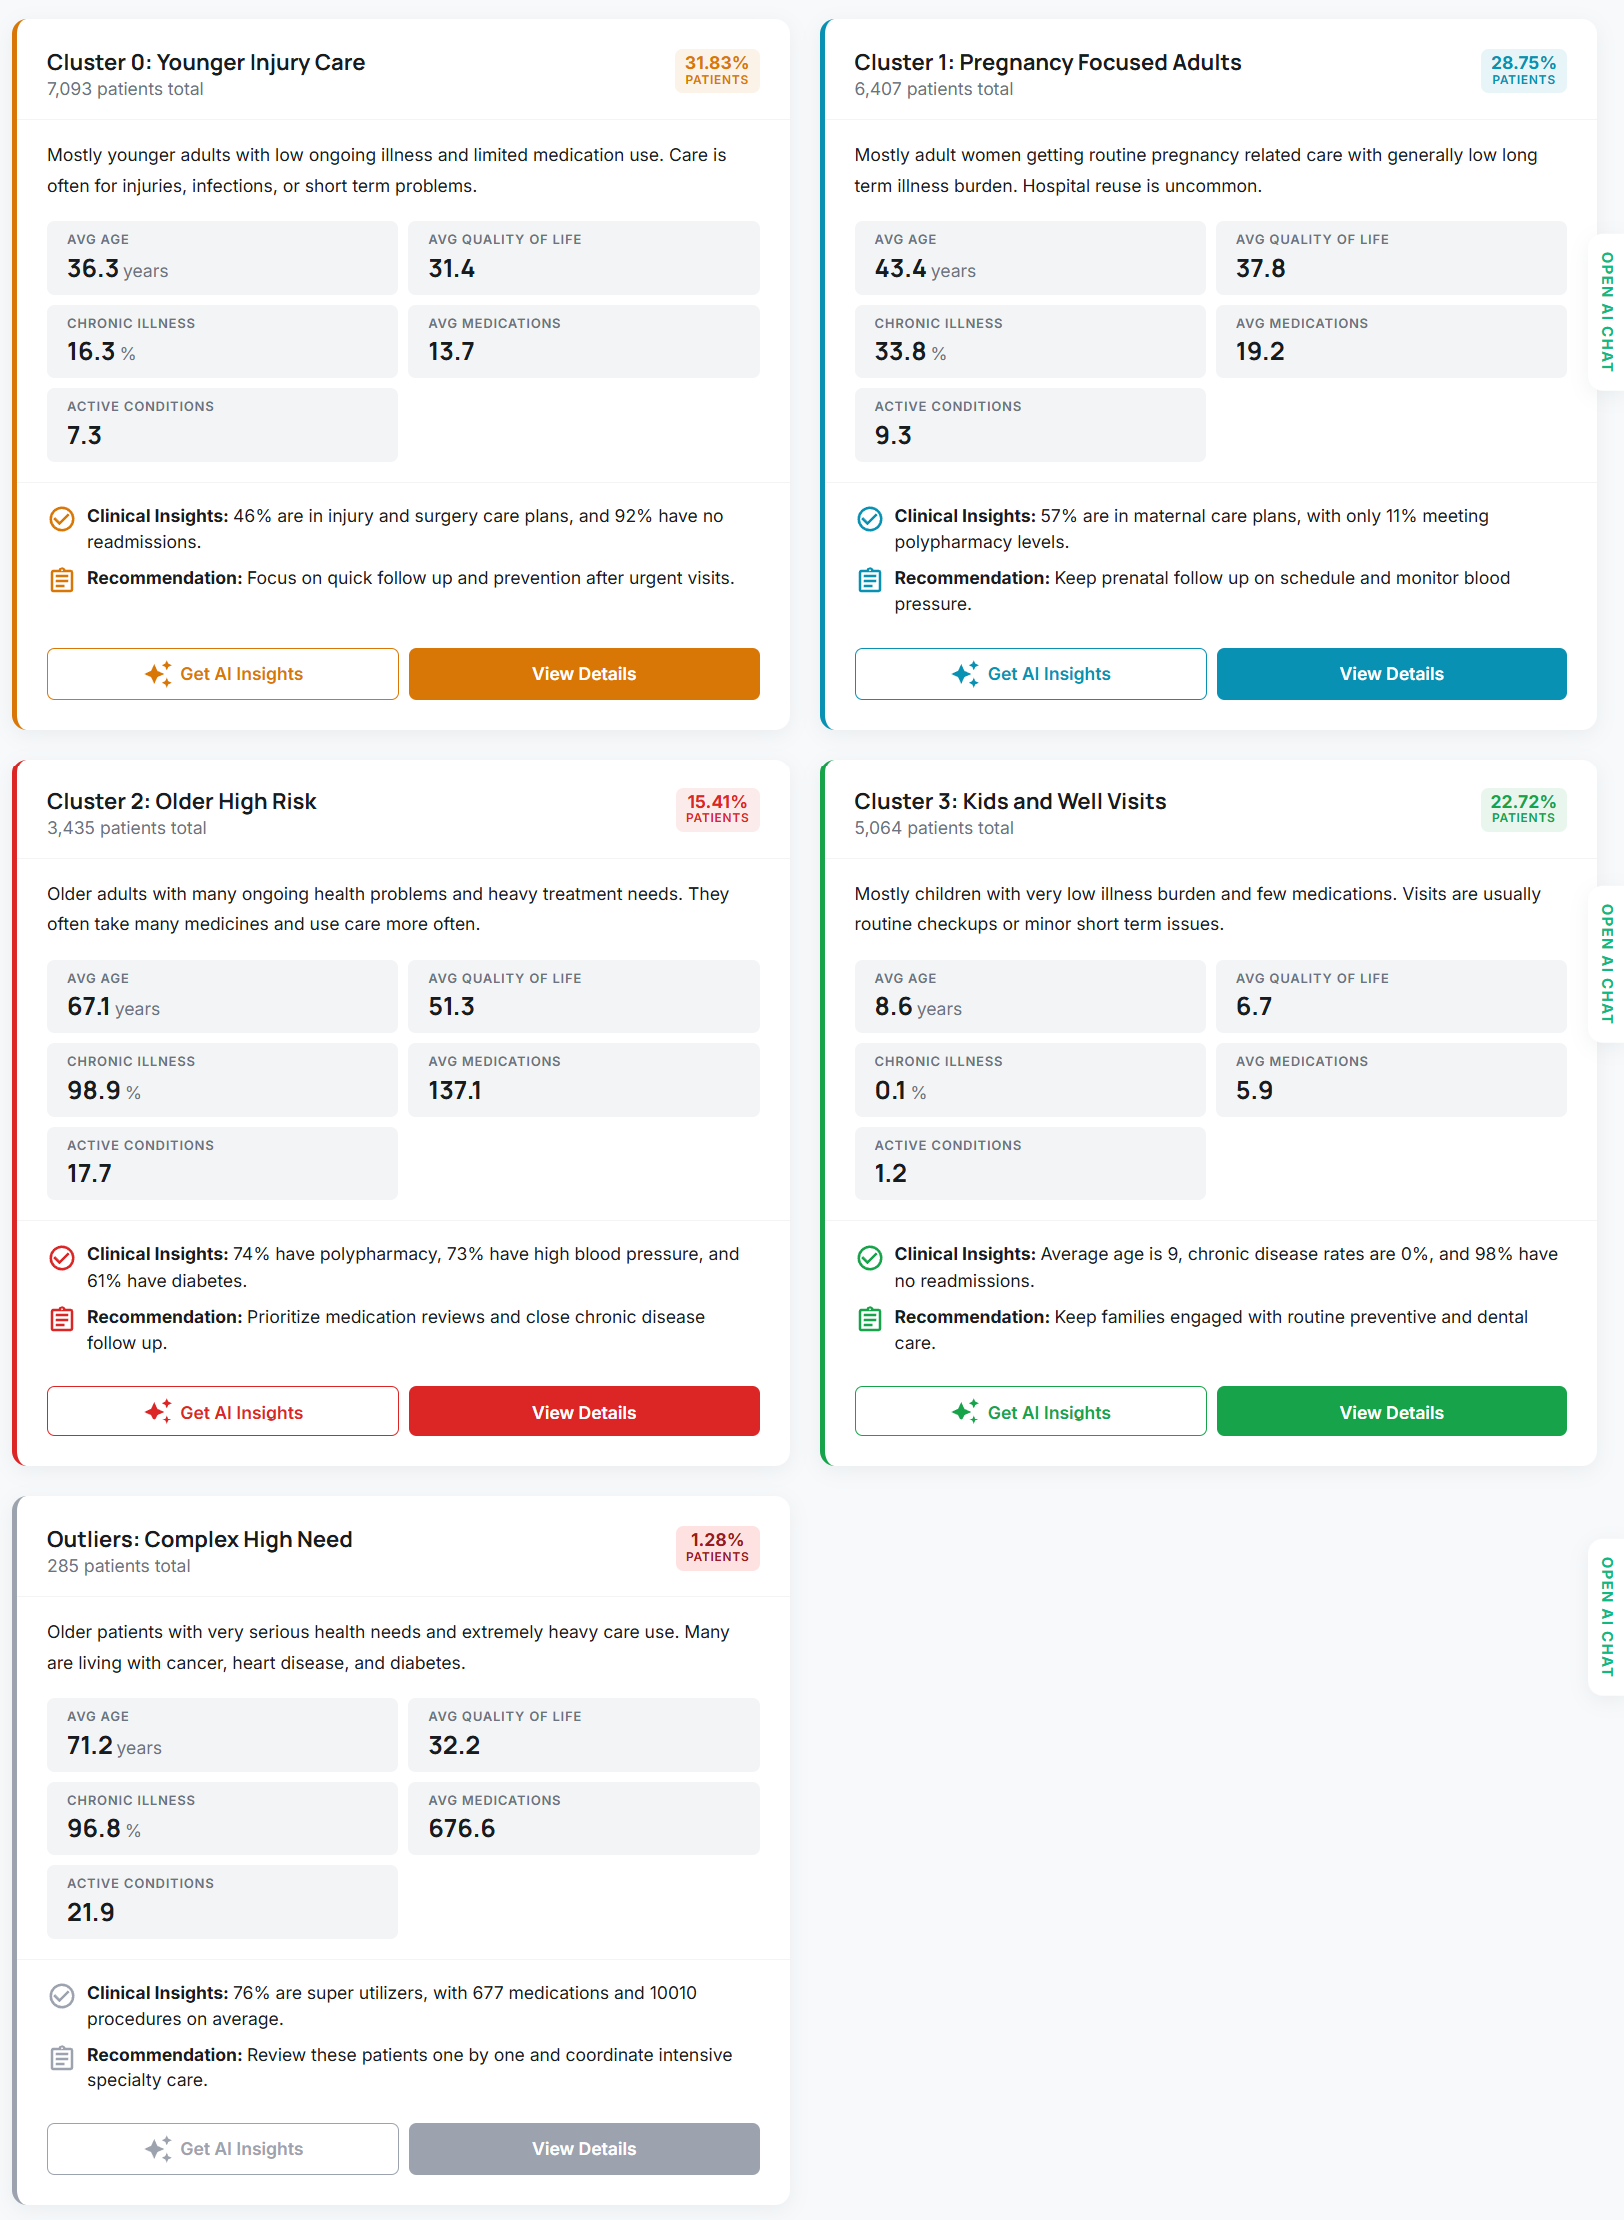
\includegraphics[width=\linewidth]{figs/platform_clusters.png}

\caption{The clusters as shown in the platform. The title, colour, description, insight and recommendation of each card are produced automatically by the AI when the clustering script runs.}

\label{fig:platform_clusters}

\end{figure}

Above and beyond the card information, the platform generates a more detailed report about every identified cluster or pattern using the mining algorithm, which has dual purposes to serve, one, as a clinical explanation intended for clinicians, and another, as a simpler, layman's summary for someone who lacks a medical perspective. This kind of explanation is depicted in Figure~\ref{fig:platform_interpretation}.

\begin{figure}[t]

\centering

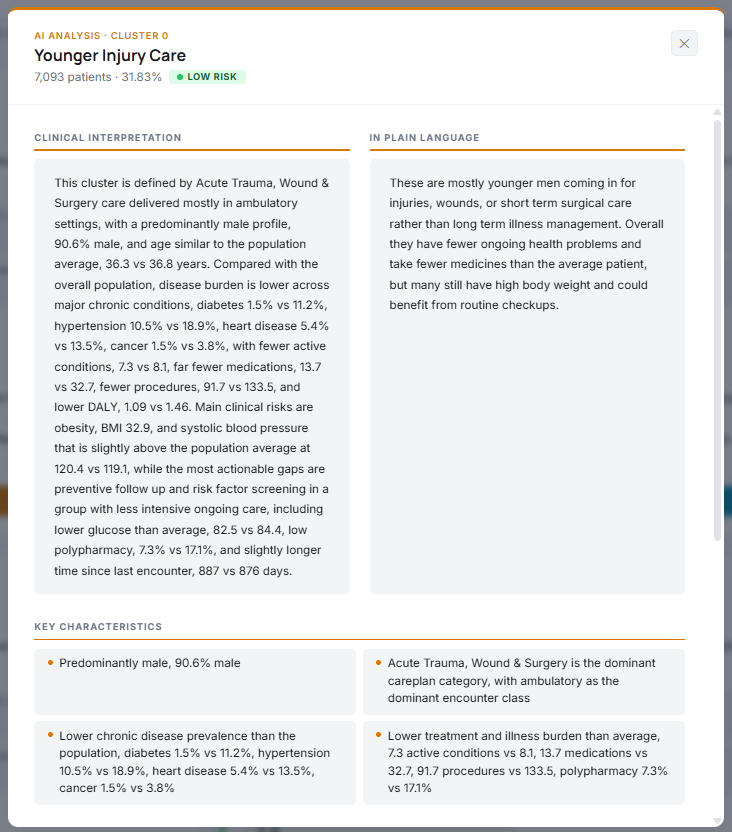
\includegraphics[width=\linewidth]{figs/platform_interpretation.png}

\caption{A cluster AI interpretation in the front end, written for both a clinician and a reader without medical training.}

\label{fig:platform_interpretation}

\end{figure}

Finally, the natural-language-to-SQL agent lets a user ask free questions. We tested it on questions of different difficulty, including non-trivial ones that need several joins. Table~\ref{tab:agent_example} lists two such questions: the first joins several clinical tables, the second joins the cluster and the sequence-mining tables. The answers are correct almost every time, and the guard layer blocked every attempt to run a non-\texttt{SELECT} statement. When the agent cannot build a valid query or finds no matching data, it plainly says it could not complete the task instead of inventing an answer.

\begin{table}[t]

\caption{Two example exchanges with the natural-language-to-SQL agent. The first needs several joins across the clinical tables, while the second joins the cluster and the sequence-mining tables.}

\label{tab:agent_example}

\centering

\footnotesize

\begin{tabular}{@{}p{0.48\linewidth}p{0.44\linewidth}@{}}

\toprule

Question & Agent answer \\

\midrule

How many distinct female patients over 60 with a diabetes diagnosis were also prescribed metformin and had at least one emergency encounter? & There were 144 distinct female patients over 60 with a diabetes diagnosis who were prescribed metformin and had at least one emergency encounter. \\[4pt]

Which mined care pathway is followed by the most patients in cluster~2, and how many of them follow it? & In cluster~2, the most common mined pathway is ``M:sodium fluoride 0.0272 MG/MG Oral Gel $\rightarrow$ P:Dental fluoride treatment $\rightarrow$ P:Oral health education'', followed by 1{,}265 patients. \\

\bottomrule

\end{tabular}

\end{table}

A full quantitative evaluation of the agent and of the generated summaries is left for future work, as discussed next.

